
\documentclass[aspectratio=169, handout, t]{beamer}

%\usepackage[table]{xcolor}
\mode<presentation> {
\setbeamercovered{transparent}
  \usetheme{Boadilla}

%  \usetheme{Pittsburgh}
%\usefonttheme[2]{sans}
\renewcommand{\familydefault}{cmss}
%\usepackage{lmodern}
%\usepackage[T1]{fontenc}
%\usepackage{palatino}
%\usepackage{cmbright}
\usepackage{bm}
\usepackage{stackrel}
\usepackage{array}
\usepackage{listings}
\useinnertheme{rectangles}
}
\usepackage{amsmath}
\setbeamercolor{normal text}{fg=black}
\setbeamercolor{structure}{fg= blue}
\definecolor{trial}{cmyk}{1,0,0, 0}
\definecolor{trial2}{cmyk}{0.00,0,1, 0}
\definecolor{darkgreen}{rgb}{0,.4, 0.1}
\usepackage{array}
\definecolor{alertpurple}{rgb}{0.4, 0, 0.6}
\beamertemplatesolidbackgroundcolor{white}  \setbeamercolor{alerted
text}{fg=alertpurple}
\usepackage{tcolorbox}
\setbeamertemplate{caption}[numbered]\newcounter{mylastframe}

\font\domino=domino
\def\die#1{{\domino#1}}
\usepackage{tikz}
\usetikzlibrary{calc}
\usetikzlibrary{arrows}
\usepackage{colortbl}

\renewcommand{\familydefault}{cmss}
%\usepackage[all]{xy}

\usepackage{tikz}
\usepackage{lipsum}
\usepackage{pgfplots}
\pgfplotsset{compat=1.17}
\usepackage{booktabs}

\lstset{%
  language=R,
  basicstyle=\ttfamily\small,
  keywordstyle=\color{blue},
  commentstyle=\color{darkgreen},
  stringstyle=\color{red},
  showstringspaces=false,
  breaklines=true,
  frame=single,
  backgroundcolor=\color{gray!10}
}

 \newenvironment{changemargin}[3]{%
 \begin{list}{}{%
 \setlength{\topsep}{0pt}%
 \setlength{\leftmargin}{#1}%
 \setlength{\rightmargin}{#2}%
 \setlength{\topmargin}{#3}%
 \setlength{\listparindent}{\parindent}%
 \setlength{\itemindent}{\parindent}%
 \setlength{\parsep}{\parskip}%
 }%
\item[]}{\end{list}}
\usetikzlibrary{arrows}

\usecolortheme{lily}

\newtheorem{com}{Comment}
\newtheorem{lem} {Lemma}
\newtheorem{prop}{Proposition}
\newtheorem{condition}{Condition}
\newtheorem{thm}{Theorem}
\newtheorem{defn}{Definition}
\newtheorem{cor}{Corollary}
\newtheorem{obs}{Observation}
 \numberwithin{equation}{section}

\makeatletter
\def\beamerorig@set@color{%
  \pdfliteral{\current@color}%
  \aftergroup\reset@color
}
\def\beamerorig@reset@color{\pdfliteral{\current@color}}
\makeatother
\setbeamertemplate{navigation symbols}{}

\useoutertheme{miniframes}
\title[PLSC 30700]{Linear Models Lecture 9: Probit and Poisson QMLE}

\author{Robert Gulotty}
\institute[Chicago]{University of Chicago}
\vspace{0.3in}

\pgfmathdeclarefunction{normalpdf}{3}{%
  \pgfmathparse{1/(#3*sqrt(2*pi))*exp(-((#1)-(#2))^2/(2*(#3)^2))}%
}
\begin{document}

\begin{frame}
\maketitle
\end{frame}

%%%%%%%%%%%%%%%%%%%%%%%%%%%%%%%%%%%%%%%%%%%%%%%%%%%%%%%%%%%%
\section{Binary Outcomes and LPM}
%%%%%%%%%%%%%%%%%%%%%%%%%%%%%%%%%%%%%%%%%%%%%%%%%%%%%%%%%%%%

\begin{frame}{Binary Outcomes and the BLP}

Recall from Lecture 2, the \textbf{best linear predictor} (BLP):
\[
\beta = \arg\min_b \, \mathbb{E}\left[(Y - X'b)^2\right]
\]

\pause

\textbf{What happens when $Y \in \{0,1\}$?}

\pause

The conditional expectation function is now a probability:
\[
m(x) = \mathbb{E}[Y \mid X = x] = P(Y = 1 \mid X = x)
\]

\pause

The BLP still exists --- OLS estimates $\beta$ by solving the same normal equations:
\[
\sum_{i=1}^n X_i(Y_i - X_i'\hat\beta) = 0
\]

This is the \textbf{linear probability model} (LPM).

\end{frame}

%%%%%%%%%%%%%%%%%%%%%%%%%%%%%%%%%%%%%%%%%%%%%%%%%%%%%%%%%%%%

\begin{frame}{LPM: Consistent for Average Marginal Effects}

Even if the true CEF $P(Y=1 \mid X)$ is nonlinear, OLS estimates a useful object.

\pause

Recall the BLP--CEF distinction from Lecture 2:
\begin{itemize}
    \item The BLP $X'\beta$ need not equal the CEF $m(x)$
    \item But $\beta$ is consistent for the \textbf{average marginal effect} under mild conditions
\end{itemize}

\pause

\textbf{Built-in heteroskedasticity} (recall Lecture 6):

If $Y_i \in \{0,1\}$, then
\[
\operatorname{Var}(Y_i \mid X_i) = p(X_i)(1 - p(X_i))
\]
where $p(X_i) = P(Y_i = 1 \mid X_i)$.

\pause

The variance depends on $X_i$ by construction. The LPM \textbf{always} requires heteroskedasticity-robust standard errors (HC2).

\end{frame}

%%%%%%%%%%%%%%%%%%%%%%%%%%%%%%%%%%%%%%%%%%%%%%%%%%%%%%%%%%%%

\begin{frame}{Limitations of the Linear Probability Model}
\begin{columns}
\begin{column}{0.48\textwidth}
\textbf{Problems:}
\begin{itemize}
    \item Predictions outside $[0,1]$
    \item Poor approximation in tails
    \item Marginal effects constant (may be unrealistic)
\end{itemize}

\pause

\textbf{Motivation:} A model that respects the $[0,1]$ constraint.

\pause

\textbf{Single-index model:}
\[
P(Y = 1 \mid X) = G(X'\beta)
\]
where $G: \mathbb{R} \to [0,1]$ is a known link function.

\end{column}
\begin{column}{0.48\textwidth}

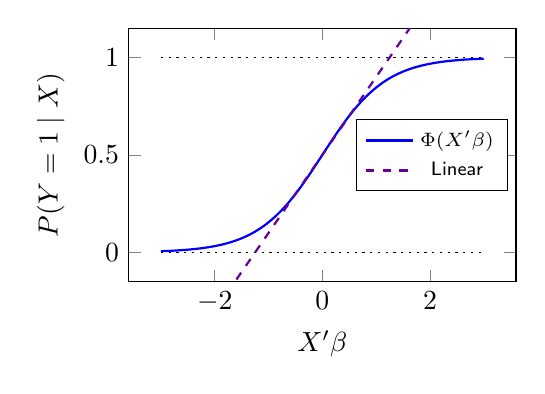
\begin{tikzpicture}
\begin{axis}[
  width=6.5cm, height=4.8cm,
  domain=-3:3, samples=100,
  xlabel={$X'\beta$}, ylabel={$P(Y=1 \mid X)$},
  ymin=-0.15, ymax=1.15,
  legend style={at={(0.98,0.5)}, anchor=east, font=\scriptsize},
  every axis plot/.append style={thick}
]
\addplot[blue] {1/(1+exp(-1.7*x))};
\addlegendentry{$\Phi(X'\beta)$}
\addplot[alertpurple, dashed] {0.5 + 0.4*x};
\addlegendentry{Linear}
\addplot[black, dotted, thin] coordinates {(-3,0)(3,0)};
\addplot[black, dotted, thin] coordinates {(-3,1)(3,1)};
\end{axis}
\end{tikzpicture}

\end{column}
\end{columns}

\end{frame}

%%%%%%%%%%%%%%%%%%%%%%%%%%%%%%%%%%%%%%%%%%%%%%%%%%%%%%%%%%%%

\begin{frame}{From LPM to Probit}

\textbf{Two common link functions:}

\medskip

\begin{tabular}{lll}
\textbf{Probit:} & $G = \Phi$ & (standard normal CDF) \\
\textbf{Logit:} & $G = \Lambda$ & (logistic CDF: $e^x/(1+e^x)$)
\end{tabular}

\pause

\bigskip

Both map $\mathbb{R} \to (0,1)$, are symmetric about $1/2$, and produce nearly identical fitted values.

\pause

\bigskip

\textbf{Why Probit?}
\begin{itemize}
    \item Natural latent variable interpretation ($\varepsilon \sim N(0,1)$)
    \item Connects to the normal distribution theory from Lectures 1 and 7
    \item Extends naturally to other nonlinear models (Poisson QMLE, later today)
\end{itemize}

\end{frame}

%%%%%%%%%%%%%%%%%%%%%%%%%%%%%%%%%%%%%%%%%%%%%%%%%%%%%%%%%%%%
\section{The Probit Model}
%%%%%%%%%%%%%%%%%%%%%%%%%%%%%%%%%%%%%%%%%%%%%%%%%%%%%%%%%%%%

\begin{frame}{Latent Variable Representation}

Suppose there exists an unobserved variable:
\[
Y_i^* = X_i'\beta + \varepsilon_i
\]

\pause

Observed outcome:
\[
Y_i = \mathbf{1}\{Y_i^* > 0\}
\]

\pause

Assume $\varepsilon_i \sim N(0,1)$. Then:\pause
\[
P(Y_i=1 \mid X_i)
=
P(\varepsilon_i > -X_i'\beta)
=
\Phi(X_i'\beta)
\]

\pause

This is the \textbf{Probit model}.
\end{frame}

%%%%%%%%%%%%%%%%%%%%%%%%%%%%%%%%%%%%%%%%%%%%%%%%%%%%%%%%%%%%

\begin{frame}{Identification and Scale Normalization}

In the latent model $Y_i^* = X_i'\beta + \varepsilon_i$, $\varepsilon_i \sim N(0,\sigma^2)$:\pause
\[
P(Y_i=1 \mid X_i)
=
\Phi\left(\frac{X_i'\beta}{\sigma}\right)
\]

\pause

Only $\beta/\sigma$ is identified --- the data cannot distinguish $(\beta, \sigma)$ from $(c\beta, c\sigma)$.

\pause

\textbf{Normalization:} Set $\operatorname{Var}(\varepsilon_i) = 1$.

\pause

\begin{tcolorbox}[colback=blue!5, colframe=blue!50, title=Key Point]
Probit coefficients are identified only up to scale. We cannot interpret $\beta_j$ the same way as in OLS. This is fundamentally different from the linear model.
\end{tcolorbox}

\end{frame}

%%%%%%%%%%%%%%%%%%%%%%%%%%%%%%%%%%%%%%%%%%%%%%%%%%%%%%%%%%%%

\begin{frame}{Marginal Effects}

In the linear model: $\partial \mathbb{E}[Y \mid X]/\partial x_j = \beta_j$.

\pause

In the Probit model:
\[
\frac{\partial P(Y=1 \mid X)}{\partial x_j}
=
\phi(X'\beta) \cdot \beta_j
\]

\pause

The marginal effect \textbf{depends on $X$} through $\phi(X'\beta)$.

\pause

\bigskip

\textbf{Average Marginal Effect} (AME):
\[
\widehat{\text{AME}}_j = \frac{1}{n}\sum_{i=1}^n \phi(X_i'\hat\beta)\,\hat\beta_j
\]

\pause

\begin{itemize}
    \item The AME averages over the observed distribution of $X$
    \item This is the natural analog of the OLS coefficient for binary outcomes
    \item Computing the AME requires the \textbf{delta method} (Lecture 10) for standard errors
\end{itemize}

\end{frame}

%%%%%%%%%%%%%%%%%%%%%%%%%%%%%%%%%%%%%%%%%%%%%%%%%%%%%%%%%%%%

\begin{frame}{Marginal Effects: Graphical Intuition}

\begin{center}
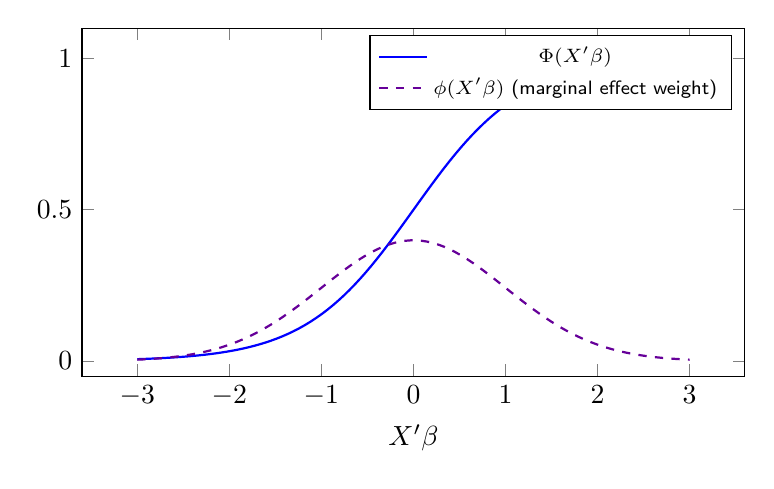
\begin{tikzpicture}
\begin{axis}[
  width=10cm, height=6cm,
  domain=-3:3, samples=100,
  xlabel={$X'\beta$}, ylabel={},
  ymin=-0.05, ymax=1.1,
  legend style={at={(0.98,0.98)}, anchor=north east, font=\scriptsize},
  every axis plot/.append style={thick}
]
% CDF (logistic approx to Phi)
\addplot[blue] {1/(1+exp(-1.7*x))};
\addlegendentry{$\Phi(X'\beta)$}
% PDF (standard normal)
\addplot[alertpurple, dashed] {exp(-x^2/2)/sqrt(2*pi)};
\addlegendentry{$\phi(X'\beta)$ (marginal effect weight)}
\end{axis}
\end{tikzpicture}
\end{center}

\pause

Marginal effects are largest near $X'\beta = 0$ (where the CDF is steepest) and vanish in the tails.

\end{frame}

%%%%%%%%%%%%%%%%%%%%%%%%%%%%%%%%%%%%%%%%%%%%%%%%%%%%%%%%%%%%
\section{MLE}
%%%%%%%%%%%%%%%%%%%%%%%%%%%%%%%%%%%%%%%%%%%%%%%%%%%%%%%%%%%%

\begin{frame}{Likelihood for the Probit Model}

Recall from Lecture 7: we developed the general MLE framework under normality. Now we apply it to a \textbf{nonlinear} model.

\pause

\bigskip

Assuming conditional independence, the likelihood is:

\[
L_n(\beta)
=
\prod_{i=1}^n
\Phi(X_i'\beta)^{Y_i}
\left(1-\Phi(X_i'\beta)\right)^{1-Y_i}
\]

\pause

Log-likelihood:

\[
\ell_n(\beta)
=
\sum_{i=1}^n
\left[
Y_i \log \Phi(X_i'\beta)
+
(1-Y_i)\log\left(1-\Phi(X_i'\beta)\right)
\right]
\]

\pause

We estimate $\hat\beta_{\text{MLE}} = \arg\max_\beta \, \ell_n(\beta)$.

\end{frame}

%%%%%%%%%%%%%%%%%%%%%%%%%%%%%%%%%%%%%%%%%%%%%%%%%%%%%%%%%%%%

\begin{frame}{Score Function}

Let $\phi(\cdot)$ denote the standard normal pdf, $\Phi(\cdot)$ the CDF.

\pause

The individual score contribution:

\[
s_i(\beta) = \frac{\partial \ell_i}{\partial \beta}
=
\frac{\phi(X_i'\beta)}{\Phi(X_i'\beta)(1-\Phi(X_i'\beta))}
\left(Y_i - \Phi(X_i'\beta)\right) X_i
\]

\pause

The total score:

\[
S_n(\beta) = \sum_{i=1}^n s_i(\beta) = \sum_{i=1}^n w_i \left(Y_i - \Phi(X_i'\beta)\right) X_i
\]

where $w_i = \phi(X_i'\beta)/[\Phi(X_i'\beta)(1-\Phi(X_i'\beta))]$.

\pause

\bigskip

Setting $S_n(\hat\beta) = 0$ defines the MLE. This is a \textbf{nonlinear} system --- no closed-form solution.

\end{frame}

%%%%%%%%%%%%%%%%%%%%%%%%%%%%%%%%%%%%%%%%%%%%%%%%%%%%%%%%%%%%

\begin{frame}[fragile]{Score in Practice: What \texttt{glm()} Solves}
\small
\begin{lstlisting}
probit <- glm(Y ~ X1 + X2, data = dta,
              family = binomial(link = "probit"))
# Compute the score at the MLE (should be ~0)
xb  <- predict(probit, type = "link")
w   <- dnorm(xb) / (pnorm(xb) * (1 - pnorm(xb)))
res <- dta$Y - pnorm(xb)           # Y_i - Phi(X'beta)
score <- colSums(w * res * model.matrix(probit))
round(score, 10)
#  (Intercept)       X1       X2
#            0        0        0
\end{lstlisting}\pause
\vspace{-2pt}
\begin{tcolorbox}[colback=blue!5, colframe=blue!50, boxsep=2pt, top=2pt, bottom=2pt]
The score is what \texttt{glm()} drives to zero.  It is the nonlinear analog of the OLS normal equations $\bm{X'}\hat{\bm{e}}=0$.
\end{tcolorbox}

\end{frame}

%%%%%%%%%%%%%%%%%%%%%%%%%%%%%%%%%%%%%%%%%%%%%%%%%%%%%%%%%%%%

\begin{frame}{Score as Moment Condition}

\textbf{Key insight:} Under correct specification, $\mathbb{E}[s_i(\beta_0)] = 0$.

\pause

\medskip

Compare three estimating equations side by side:

\smallskip

\renewcommand{\arraystretch}{1.6}
\begin{tabular}{lll}
\toprule
\textbf{Model} & \textbf{Estimating Equation} & \textbf{Mean Function} \\
\midrule
OLS & $\displaystyle\sum_i X_i(Y_i - X_i'\beta) = 0$ & $X'\beta$ \\[6pt]
Probit MLE & $\displaystyle\sum_i w_i(Y_i - \Phi(X_i'\beta))\, X_i = 0$ & $\Phi(X'\beta)$ \\[6pt]
Poisson QMLE & $\displaystyle\sum_i X_i(Y_i - \exp(X_i'\beta)) = 0$ & $\exp(X'\beta)$ \\[6pt]
\bottomrule
\end{tabular}
\renewcommand{\arraystretch}{1.0}

\pause

\smallskip

All three are \textbf{moment conditions}: find $\theta$ s.t.\ $\frac{1}{n}\sum_i g(W_i, \theta) = 0$ (GMM).

\end{frame}

%%%%%%%%%%%%%%%%%%%%%%%%%%%%%%%%%%%%%%%%%%%%%%%%%%%%%%%%%%%%

\begin{frame}{Iterative Estimation: Newton--Raphson}

Unlike OLS, the Probit MLE has no closed-form solution.

\pause

\textbf{Newton--Raphson} iterates:
\[
\beta^{(t+1)} = \beta^{(t)} - \left[H_n(\beta^{(t)})\right]^{-1} S_n(\beta^{(t)})
\]

where $H_n(\beta) = \partial S_n / \partial \beta' = \partial^2 \ell_n / \partial \beta \partial \beta'$ is the Hessian.

\pause

\bigskip

\textbf{Algorithm:}
\begin{enumerate}
    \item Start with an initial guess $\beta^{(0)}$ (e.g., OLS estimates)
    \item Compute score $S_n(\beta^{(t)})$ and Hessian $H_n(\beta^{(t)})$
    \item Update: $\beta^{(t+1)} = \beta^{(t)} - H_n^{-1} S_n$
    \item Repeat until convergence: $\|\beta^{(t+1)} - \beta^{(t)}\| < \varepsilon$
\end{enumerate}

\pause

In practice, \texttt{glm()} in R handles this automatically via Fisher scoring (a variant of Newton--Raphson).

\end{frame}

%%%%%%%%%%%%%%%%%%%%%%%%%%%%%%%%%%%%%%%%%%%%%%%%%%%%%%%%%%%%

\begin{frame}[fragile]{Newton--Raphson in Practice: Watching \texttt{glm()} Iterate}

\begin{lstlisting}
probit <- glm(Y ~ X1 + X2, data = dta,
              family = binomial(link = "probit"),
              control = list(trace = TRUE))
# Deviance = -2 * log-likelihood (lower = better)
#   Deviance = 134.60 Iterations - 1
#   Deviance = 130.28 Iterations - 2
#   Deviance = 130.21 Iterations - 3
#   Deviance = 130.21 Iterations - 4   <- converged
\end{lstlisting}\pause

\begin{itemize}
\item Each iteration applies the Newton--Raphson update $\beta^{(t+1)} = \beta^{(t)} - H^{-1}S$.\pause
\item Convergence is typically fast (3--6 iterations) because the log-likelihood is concave.\pause
\item If \texttt{glm()} warns ``algorithm did not converge,'' the score could not be driven to zero --- a sign of separation or misspecification.
\end{itemize}

\end{frame}

%%%%%%%%%%%%%%%%%%%%%%%%%%%%%%%%%%%%%%%%%%%%%%%%%%%%%%%%%%%%

\begin{frame}{Why Not Just Use OLS?}

\begin{center}
\renewcommand{\arraystretch}{1.3}
\small
\begin{tabular}{lcc}
\toprule
& \textbf{LPM (OLS)} & \textbf{Probit (MLE)} \\
\midrule
Closed-form solution & Yes & No \\
Predictions in $[0,1]$ & Not guaranteed & Yes \\
Consistent for $\beta$ & --- & Yes (if correctly specified) \\
Consistent for AME & Yes (always) & Yes (if correctly specified) \\
Robust to misspecification & Yes (BLP always exists) & Requires sandwich SEs \\
Efficiency & Lower & Higher (if correct) \\
\bottomrule
\end{tabular}
\renewcommand{\arraystretch}{1.0}
\normalsize
\end{center}

\pause

\begin{tcolorbox}[colback=blue!5, colframe=blue!50, boxsep=2pt, top=2pt, bottom=2pt]
\textbf{Practical guidance:} LPM is a robust baseline. Probit gains efficiency if the model is correct, but misspecification has consequences.
\end{tcolorbox}

\end{frame}

%%%%%%%%%%%%%%%%%%%%%%%%%%%%%%%%%%%%%%%%%%%%%%%%%%%%%%%%%%%%
\section{Asymptotics}
%%%%%%%%%%%%%%%%%%%%%%%%%%%%%%%%%%%%%%%%%%%%%%%%%%%%%%%%%%%%

\begin{frame}{Fisher Information for Probit}

The Fisher information matrix is:
\[
\mathcal{I}(\beta)
=
\mathbb{E}\left[\frac{\phi(X'\beta)^2}{\Phi(X'\beta)(1-\Phi(X'\beta))} \, XX'\right]
\]

\pause

\textbf{Derivation:} By the information matrix equality,
\[
\mathcal{I}(\beta) = \mathbb{E}[s_i(\beta) s_i(\beta)'] = -\mathbb{E}\left[\frac{\partial^2 \ell_i(\beta)}{\partial \beta \partial \beta'}\right]
\]

\pause

The weight $\frac{\phi(X'\beta)^2}{\Phi(X'\beta)(1-\Phi(X'\beta))}$ is largest when $X'\beta \approx 0$ (where we have the most ``information'' about $\beta$) and smallest in the tails.

\pause

\bigskip

Compare with OLS: $\mathbb{E}[X X'] / \sigma^2$. In Probit, the effective ``variance'' changes with $X$.

\end{frame}

%%%%%%%%%%%%%%%%%%%%%%%%%%%%%%%%%%%%%%%%%%%%%%%%%%%%%%%%%%%%

\begin{frame}{Hessian and Outer Product of Scores}

The expected Hessian:
\[
-\mathbb{E}\!\left[\frac{\partial^2 \ell_i}{\partial \beta \partial \beta'}\right]
=
\mathbb{E}\!\left[\frac{\phi(X'\beta)^2}{\Phi(X'\beta)(1-\Phi(X'\beta))} X X'\right]
\]

\pause

\bigskip

The outer product of scores:
\[
\mathbb{E}[s_i s_i']
=
\mathbb{E}\!\left[\frac{\phi(X'\beta)^2}{\Phi(X'\beta)^2(1-\Phi(X'\beta))^2} \underbrace{(Y_i - \Phi)^2}_{\Phi(1-\Phi)} X X'\right]
\]

\pause

\bigskip

These two expressions \emph{look} different. Are they equal?

\end{frame}

%%%%%%%%%%%%%%%%%%%%%%%%%%%%%%%%%%%%%%%%%%%%%%%%%%%%%%%%%%%%

\begin{frame}{Information Matrix Equality}

Since $\mathbb{E}[(Y_i - \Phi)^2 \mid X_i] = \Phi(1-\Phi)$, one factor of $\Phi(1-\Phi)$ in the denominator cancels:

\[
\mathbb{E}[s_i s_i']
=
\mathbb{E}\!\left[\frac{\phi(X'\beta)^2}{\Phi(X'\beta)(1-\Phi(X'\beta))} X X'\right]
= -\mathbb{E}\!\left[\frac{\partial^2 \ell_i}{\partial \beta \partial \beta'}\right]
\]

\pause

\bigskip

This gives the \textbf{information matrix equality} (under correct specification):
\[
\boxed{\mathbb{E}[s_i s_i'] = -\mathbb{E}\!\left[\frac{\partial^2 \ell_i}{\partial \beta \partial \beta'}\right]}
\]

\pause

\bigskip

When this equality holds, model-based SEs and sandwich SEs agree. When it fails (misspecification), only the sandwich is valid.

\end{frame}

%%%%%%%%%%%%%%%%%%%%%%%%%%%%%%%%%%%%%%%%%%%%%%%%%%%%%%%%%%%%

\begin{frame}[fragile]{From Fisher Information to the SEs You See in R}

\texttt{summary(glm(...))} reports standard errors.  Where do they come from?\pause

\begin{lstlisting}
# Model-based SEs = sqrt of diagonal of inverse Hessian
sqrt(diag(vcov(probit)))
#  (Intercept)       X1        X2
#     0.241       0.058     0.103

# These are the SEs in summary() output
summary(probit)$coefficients[, "Std. Error"]
#     same numbers
\end{lstlisting}\pause

\begin{itemize}
\item \texttt{vcov(probit)} $= \hat{\mathcal{H}}^{-1} = \left[-\frac{1}{n}\sum_i \frac{\partial^2 \ell_i}{\partial \beta \partial \beta'}\right]^{-1}$\pause
\item Under correct specification, $\hat{\mathcal{H}}^{-1} = \hat{\mathcal{I}}^{-1}$ (information equality), so one matrix suffices.\pause
\item Under misspecification, you need the sandwich: \texttt{vcovHC(probit)} $= \hat{\mathcal{H}}^{-1}\hat{\mathcal{I}}\,\hat{\mathcal{H}}^{-1}$.
\end{itemize}

\end{frame}

%%%%%%%%%%%%%%%%%%%%%%%%%%%%%%%%%%%%%%%%%%%%%%%%%%%%%%%%%%%%

\begin{frame}{Asymptotic Normality: Derivation Sketch}

Taylor-expand the score around $\beta_0$:
\[
0 = S_n(\hat\beta) \approx S_n(\beta_0) + H_n(\beta_0)(\hat\beta - \beta_0)
\]

\pause

Rearranging:
\[
\sqrt{n}(\hat\beta - \beta_0) \approx \left[-\frac{1}{n}H_n(\beta_0)\right]^{-1} \frac{1}{\sqrt{n}} S_n(\beta_0)
\]

\pause

By the law of large numbers: $\frac{1}{n}H_n(\beta_0) \overset{p}{\to} -\mathcal{I}(\beta_0)$.

\pause

By the CLT: $\frac{1}{\sqrt{n}} S_n(\beta_0) \overset{d}{\to} N(0, \mathcal{I}(\beta_0))$.

\pause

Combining:
\[
\boxed{\sqrt{n}(\hat\beta - \beta_0) \overset{d}{\to} N\!\left(0,\; \mathcal{I}(\beta_0)^{-1}\right)}
\]

\pause

Same structure as Lecture 7, but now for a nonlinear model. The asymptotic tools (WLLN, CLT) will be developed formally in Lecture 10.

\end{frame}

%%%%%%%%%%%%%%%%%%%%%%%%%%%%%%%%%%%%%%%%%%%%%%%%%%%%%%%%%%%%

\begin{frame}{The Sandwich Under Misspecification}

\textbf{What if $\Phi$ is the wrong link function?}

\pause

If the true CEF is $G_0(X'\beta)$ but we estimate Probit, the information matrix equality \textbf{fails}:
\[
\mathbb{E}[s_i s_i'] \neq -\mathbb{E}\!\left[\frac{\partial^2 \ell_i}{\partial \beta \partial \beta'}\right]
\]

\pause

The asymptotic variance becomes the \textbf{sandwich} (recall Lectures 5--6):
\[
\operatorname{Var}(\sqrt{n}(\hat\beta - \beta_0))
=
\underbrace{H^{-1}}_{\text{bread}}
\underbrace{\mathbb{E}[s_i s_i']}_{\text{meat}}
\underbrace{H^{-1}}_{\text{bread}}
\]

where $H = -\mathbb{E}[\partial^2 \ell_i / \partial\beta\partial\beta']$.

\pause

\textbf{Quasi-MLE} (QMLE): Even with the wrong $G$, the index $X'\beta$ can be consistently estimated (up to scale) --- a form of semi-parametric resilience.

\pause

\textbf{Practical implication:} Use robust (sandwich) SEs for Probit, just as for OLS. Same \texttt{sandwich} package in R. \textit{(HW4 Q2 fits a probit IRT on UN votes.)}

\end{frame}

%%%%%%%%%%%%%%%%%%%%%%%%%%%%%%%%%%%%%%%%%%%%%%%%%%%%%%%%%%%%
\section{Poisson QMLE}
%%%%%%%%%%%%%%%%%%%%%%%%%%%%%%%%%%%%%%%%%%%%%%%%%%%%%%%%%%%%

\begin{frame}{From Binary to Nonnegative Outcomes}

Probit handles $Y \in \{0,1\}$ by passing $X'\beta$ through $\Phi$.

\pause

\textbf{What about $Y \geq 0$?} Counts, dollar amounts, rates, corner solutions.

\pause

\bigskip

Same problem as LPM: a linear model $\mathbb{E}[Y \mid X] = X'\beta$ can predict \textbf{negative values} for an outcome that cannot be negative.

\pause

\bigskip

\textbf{Solution: the exponential conditional mean.}
\[
\mathbb{E}[Y \mid X] = \exp(X'\beta)
\]

\begin{itemize}
    \item Always positive
    \item Natural for counts, corner solutions, and any $Y \geq 0$
    \item The analog of $\Phi(X'\beta)$ for binary outcomes
\end{itemize}

\end{frame}

%%%%%%%%%%%%%%%%%%%%%%%%%%%%%%%%%%%%%%%%%%%%%%%%%%%%%%%%%%%%

\begin{frame}{Why $\exp(X'\beta)$? Invariance}

Positivity is not the only reason. The exponential mean is natural when the \textbf{mechanism} implies scale invariance:\pause

\begin{itemize}
    \item \textbf{Proportional change} (population growth, compounding returns): effects should be stable under rescaling $\to$ a semi-elasticity, not an absolute change\pause
    \item \textbf{Event arrival} (conflicts, patent filings): expected counts should add when you double the observation window\pause
    \item Both imply $\mathbb{E}[Y\mid X]=\exp(X'\beta)$, not $X'\beta$
\end{itemize}

\pause

\begin{tcolorbox}[colback=blue!5, colframe=blue!50, boxsep=2pt, top=2pt, bottom=2pt]
The choice between $X'\beta$ and $\exp(X'\beta)$ is not just about the data format---it reflects a claim about what transformation of the world leaves the effect unchanged.
\end{tcolorbox}

\end{frame}

%%%%%%%%%%%%%%%%%%%%%%%%%%%%%%%%%%%%%%%%%%%%%%%%%%%%%%%%%%%%

\begin{frame}{The Poisson Quasi-Log-Likelihood}

The Poisson log-likelihood for a single observation:
\[
\ell_i(\beta) = Y_i \cdot X_i'\beta - \exp(X_i'\beta) - \log(Y_i!)
\]

\pause

The score (gradient):
\[
s_i(\beta) = \left(Y_i - \exp(X_i'\beta)\right) X_i
\]

\pause

Setting the total score to zero:
\[
\boxed{\sum_{i=1}^n X_i\left(Y_i - \exp(X_i'\beta)\right) = 0}
\]

\pause

\bigskip

Compare to OLS: $\sum X_i(Y_i - X_i'\beta) = 0$.

\medskip

Same structure --- a \textbf{nonlinear moment condition}. No observation-specific weights (unlike probit).

\end{frame}

%%%%%%%%%%%%%%%%%%%%%%%%%%%%%%%%%%%%%%%%%%%%%%%%%%%%%%%%%%%%

\begin{frame}{QMLE: Consistency Without the Distribution}

\begin{tcolorbox}[colback=blue!5, colframe=blue!50, title=Key Result (Gourieroux et al.~1984; Wooldridge 2010{,} 2023), boxsep=2pt, top=2pt, bottom=2pt]
Poisson QMLE is \textbf{consistent for $\beta$} whenever $\mathbb{E}[Y \mid X] = \exp(X'\beta)$ is correctly specified.
$Y$ need \textbf{not} be Poisson. It need not even be integer-valued.
\end{tcolorbox}

\pause

\smallskip

This is \textbf{quasi-MLE}: use a likelihood as an estimation device, not as a distributional assumption.

\pause

\smallskip

\textbf{What can $Y$ be?}
\begin{itemize}\setlength{\itemsep}{1pt}
    \item Integer counts (patents, murders, votes)
    \item Continuous nonneg (income, expenditure, trade flows)
    \item Corner solutions (zero with positive mass, then continuous)
    \item Fractions in $[0,\infty)$
\end{itemize}

\pause

All that matters is that the conditional mean is exponential.

\end{frame}

%%%%%%%%%%%%%%%%%%%%%%%%%%%%%%%%%%%%%%%%%%%%%%%%%%%%%%%%%%%%

\begin{frame}{Interpreting Poisson QMLE Coefficients}

Because $\mathbb{E}[Y \mid X] = \exp(X'\beta)$:
\[
\frac{\mathbb{E}[Y \mid x_j + 1,\, \mathbf{x}_{-j}]}{\mathbb{E}[Y \mid x_j,\, \mathbf{x}_{-j}]} = \exp(\beta_j)
\]

\pause

\medskip

$\beta_j$ is a \textbf{semi-elasticity}: a one-unit increase in $x_j$ changes $\mathbb{E}[Y \mid X]$ by approximately $100 \times \beta_j$ percent.

\pause

\medskip

\renewcommand{\arraystretch}{1.3}
\begin{tabular}{lll}
\toprule
\textbf{Model} & \textbf{$\beta_j$ measures} & \textbf{Interpretation} \\
\midrule
OLS & $\Delta \mathbb{E}[Y \mid X]$ & Absolute change \\
Probit & $\phi(X'\beta) \cdot \beta_j$ & Needs ME transformation \\
Poisson QMLE & $\approx 100\beta_j\%$ change & Semi-elasticity \\
\bottomrule
\end{tabular}
\renewcommand{\arraystretch}{1.0}

\pause

\medskip

Poisson coefficients are directly interpretable --- no marginal effect computation needed.

\end{frame}

%%%%%%%%%%%%%%%%%%%%%%%%%%%%%%%%%%%%%%%%%%%%%%%%%%%%%%%%%%%%

\begin{frame}{Sandwich SEs Are Mandatory}

The Poisson variance assumption: $\operatorname{Var}(Y \mid X) = \mathbb{E}[Y \mid X]$.

\pause

\medskip

This is almost \textbf{never correct} in practice. With overdispersion:
\[
\operatorname{Var}(Y \mid X) \gg \mathbb{E}[Y \mid X]
\]

\pause

The information matrix equality \textbf{fails} $\Rightarrow$ model-based SEs are wrong.

\pause

\medskip

\begin{tcolorbox}[colback=blue!5, colframe=blue!50, title=Practical Rule, boxsep=2pt, top=2pt, bottom=2pt]
\textbf{Always} use sandwich standard errors with Poisson QMLE. The model-based SEs from \texttt{summary(glm(...))} are not valid.
This is the same sandwich from Lectures 5--6, applied to a nonlinear model.
\end{tcolorbox}

\pause

\smallskip

Contrast with probit: sandwich SEs are \emph{optional} under correct specification, \textbf{mandatory} for Poisson QMLE.

\end{frame}

%%%%%%%%%%%%%%%%%%%%%%%%%%%%%%%%%%%%%%%%%%%%%%%%%%%%%%%%%%%%

\begin{frame}{The LEF Framework (Wooldridge 2023)}

\textbf{Linear exponential family} (LEF) distributions provide a unified framework:

\bigskip

\renewcommand{\arraystretch}{1.4}
\begin{tabular}{llll}
\toprule
\textbf{Cond.\ Mean} & \textbf{LEF Density} & \textbf{Outcome Type} & \textbf{R Code} \\
\midrule
Linear & Normal & Any $Y$ & \texttt{lm()} \\
Logistic & Bernoulli & Binary / fractional & \texttt{glm(, binomial)} \\
Exponential & Poisson & $Y \geq 0$, no upper bound & \texttt{glm(, poisson)} \\
\bottomrule
\end{tabular}
\renewcommand{\arraystretch}{1.0}

\pause

\bigskip

\begin{tcolorbox}[colback=blue!5, colframe=blue!50, boxsep=2pt, top=2pt, bottom=2pt]
In each case, consistency requires only that the \textbf{conditional mean} is correctly specified---not the full distribution. Use sandwich SEs in all cases.
\end{tcolorbox}

\end{frame}

%%%%%%%%%%%%%%%%%%%%%%%%%%%%%%%%%%%%%%%%%%%%%%%%%%%%%%%%%%%%

\begin{frame}{Applied Workflow}

\textbf{When estimating models for nonnegative outcomes:}

\bigskip

\begin{enumerate}
    \item Estimate OLS (linear) as a baseline
    \item Estimate Poisson QMLE (exponential mean) for $Y \geq 0$
    \item Compare estimates as a \textbf{robustness check}
    \item Use sandwich SEs in all cases
    \item If estimates diverge, investigate functional form
\end{enumerate}

\pause

\bigskip

This extends naturally to panel data (DiD with nonneg outcomes).

\end{frame}

%%%%%%%%%%%%%%%%%%%%%%%%%%%%%%%%%%%%%%%%%%%%%%%%%%%%%%%%%%%%
\section{R Implementation}
%%%%%%%%%%%%%%%%%%%%%%%%%%%%%%%%%%%%%%%%%%%%%%%%%%%%%%%%%%%%

\begin{frame}[fragile]{Probit in R: \texttt{glm()}}

\begin{lstlisting}
# Linear Probability Model
lpm <- lm(Y ~ X1 + X2, data = dta)

# Probit Model
probit <- glm(Y ~ X1 + X2, data = dta,
              family = binomial(link = "probit"))

# Compare coefficients
cbind(LPM = coef(lpm), Probit = coef(probit))
\end{lstlisting}

\pause

\bigskip

\begin{itemize}
    \item \texttt{glm()} uses Fisher scoring (iteratively reweighted least squares)
    \item \texttt{family = binomial(link = "probit")} specifies $G = \Phi$
    \item For logit: \texttt{family = binomial(link = "logit")}
\end{itemize}

\end{frame}

%%%%%%%%%%%%%%%%%%%%%%%%%%%%%%%%%%%%%%%%%%%%%%%%%%%%%%%%%%%%

\begin{frame}[fragile]{Marginal Effects in R}

Probit coefficients $\hat\beta_j$ are \textbf{not} marginal effects. Compute them manually:

\begin{lstlisting}
# Average Marginal Effect (AME)
xb <- predict(probit, type = "link")  # X'beta-hat
ame <- mean(dnorm(xb)) * coef(probit)
ame
\end{lstlisting}

\pause

\bigskip

Or using the \texttt{margins} package:

\begin{lstlisting}
library(margins)
summary(margins(probit))
\end{lstlisting}

\pause

The AME is directly comparable to the LPM coefficient --- both estimate $\mathbb{E}[\partial P / \partial x_j]$.

\end{frame}

%%%%%%%%%%%%%%%%%%%%%%%%%%%%%%%%%%%%%%%%%%%%%%%%%%%%%%%%%%%%

\begin{frame}[fragile]{Robust Standard Errors for Probit}

Same \texttt{sandwich} tools from Lecture 6:

\begin{lstlisting}
library(sandwich)
library(lmtest)

# Default (model-based) SEs
coeftest(probit)

# Robust (sandwich) SEs
coeftest(probit, vcov = vcovHC(probit, type = "HC1"))
\end{lstlisting}

\pause

\bigskip

\begin{itemize}
    \item Model-based SEs rely on the information matrix equality (correct specification)
    \item Sandwich SEs are valid even under misspecification (QMLE)
    \item If model-based and robust SEs differ substantially, this signals possible misspecification
\end{itemize}

\end{frame}

%%%%%%%%%%%%%%%%%%%%%%%%%%%%%%%%%%%%%%%%%%%%%%%%%%%%%%%%%%%%

\begin{frame}[fragile]{Poisson QMLE in R: \texttt{glm()}}

\begin{lstlisting}
# Poisson QMLE for nonnegative Y
pois <- glm(Y ~ X1 + X2, data = dta,
            family = poisson)

# MANDATORY: sandwich SEs (model-based are wrong)
coeftest(pois, vcov = vcovHC(pois, type = "HC1"))
\end{lstlisting}

\pause

\bigskip

\begin{lstlisting}
# Coefficient interpretation
exp(coef(pois))  # multiplicative effects
\end{lstlisting}

\pause

\bigskip

\begin{itemize}
    \item Works even if \texttt{Y} is continuous (non-integer) --- R warns, but estimates are valid
    \item \texttt{exp(coef(pois)["X1"])} = multiplicative effect of one-unit increase in \texttt{X1}
    \item Compare to OLS: \texttt{lm(Y \~{} X1 + X2)} as a robustness check
\end{itemize}

\end{frame}

%%%%%%%%%%%%%%%%%%%%%%%%%%%%%%%%%%%%%%%%%%%%%%%%%%%%%%%%%%%%
\section{Synthesis}
%%%%%%%%%%%%%%%%%%%%%%%%%%%%%%%%%%%%%%%%%%%%%%%%%%%%%%%%%%%%

\begin{frame}{Comparison Table}

\begin{center}
\renewcommand{\arraystretch}{1.25}
\small
\begin{tabular}{lcccc}
\toprule
& \textbf{OLS} & \textbf{LPM} & \textbf{Probit} & \textbf{Poisson QMLE} \\
\midrule
Outcome & Any & Binary & Binary & $Y \geq 0$ \\
CEF & $X'\beta$ & $X'\beta$ & $\Phi(X'\beta)$ & $\exp(X'\beta)$ \\
$\beta_j$ means & $\Delta Y$ & $\Delta P$ & needs ME & $\approx \%\Delta Y$ \\
Moment cond. & $\sum Xe = 0$ & $\sum Xe = 0$ & $\sum ws = 0$ & $\sum X(Y-e^{X'\beta})=0$ \\
Sandwich SEs & Rec. & Mandatory & Optional & \alert{Mandatory} \\
Invariance & Translation & Translation & Monotone latent & Scale \\
\bottomrule
\end{tabular}
\renewcommand{\arraystretch}{1.0}
\normalsize
\end{center}

\pause

\textbf{The GMM generalization:} All of these are special cases of
\[
\mathbb{E}[g(W_i, \theta_0)] = 0
\]

Find $\hat\theta$ such that $\frac{1}{n}\sum_{i=1}^n g(W_i, \hat\theta) \approx 0$. This is the \textbf{Generalized Method of Moments}.

\end{frame}

%%%%%%%%%%%%%%%%%%%%%%%%%%%%%%%%%%%%%%%%%%%%%%%%%%%%%%%%%%%%

\begin{frame}{Key Takeaways and Looking Ahead}

\textbf{Today:}
\begin{itemize}
    \item Binary outcomes $\Rightarrow$ Probit; nonneg outcomes $\Rightarrow$ Poisson QMLE
    \item LPM and OLS remain useful baselines for comparison
    \item Probit: $\beta_j$ needs marginal effect transformation; Poisson: $\beta_j \approx$ semi-elasticity
    \item All score equations are \textbf{moment conditions} --- nonlinear GMM
    \item Poisson QMLE: consistent if $\mathbb{E}[Y \mid X] = \exp(X'\beta)$, regardless of the distribution of $Y$
    \item Sandwich SEs: optional for probit (under correct spec), \alert{mandatory} for Poisson QMLE
    \item Always compare linear and nonlinear estimates as a robustness check
\end{itemize}

\pause

\bigskip

\textbf{Next (Lecture 10):} The formal asymptotic tools --- WLLN, CLT, delta method --- that justify everything we did today.

\end{frame}


\end{document}
